\section{Optimized Grid Model}
\setlength{\parindent}{10ex}
%Purpose of this section is to identify the optimized grid structure.
%I need to check with Hoque to identify what I should and shouldnt include
%I need to consider rewording this and restructuring to manage the correctness for example etc.
Classification results showed that groups of classes had higher prediction rates in different models.
These results support that there is a optimum classifier for a area of the ocean.
The Grid Optimized Model Injector Classifier was created to test this theory.
This model is built upon the idea that there is not a optimal single model for predicting all of the worlds bathymetry.
It leverages several different models to predict bathymetry in a area by recording the best preforming models across a grid of the world.
This allows the model to use the optimal model for predicting bathymetry.

%Give the background for the idea in this section!
\subsection{Grid Optimizing Background}
According to the "No Free Lunch Theorem" \cite{wolpert1997no}, there is no optimal model to solve all problems.
For machine learning this theorem especially holds true.
To append onto the therm, there is not a single model that will optimally predict the entire globes bathymetry.
A model that preforms well in a area of the pacific may not preform well in the Atlantic.
Earth is a large planet with vastly different environments across degrees of latitude.
Likewise, the ocean ecosystem and topography changes relative to the location on the Earth.

\par
In the classification portion of this work there was evidence that a optimum model for a coverage exists.
This coverage should be designated to maximize accurate predictions.
Therefore, a proof of concept for this model will be to divide the Earth into coverages and test a set of models against each.
This will prove that a optimal set of coverages for a model does exist, and that localizing these models will yield benefit for predictions.

\begin{figure}[h]
    \centering
    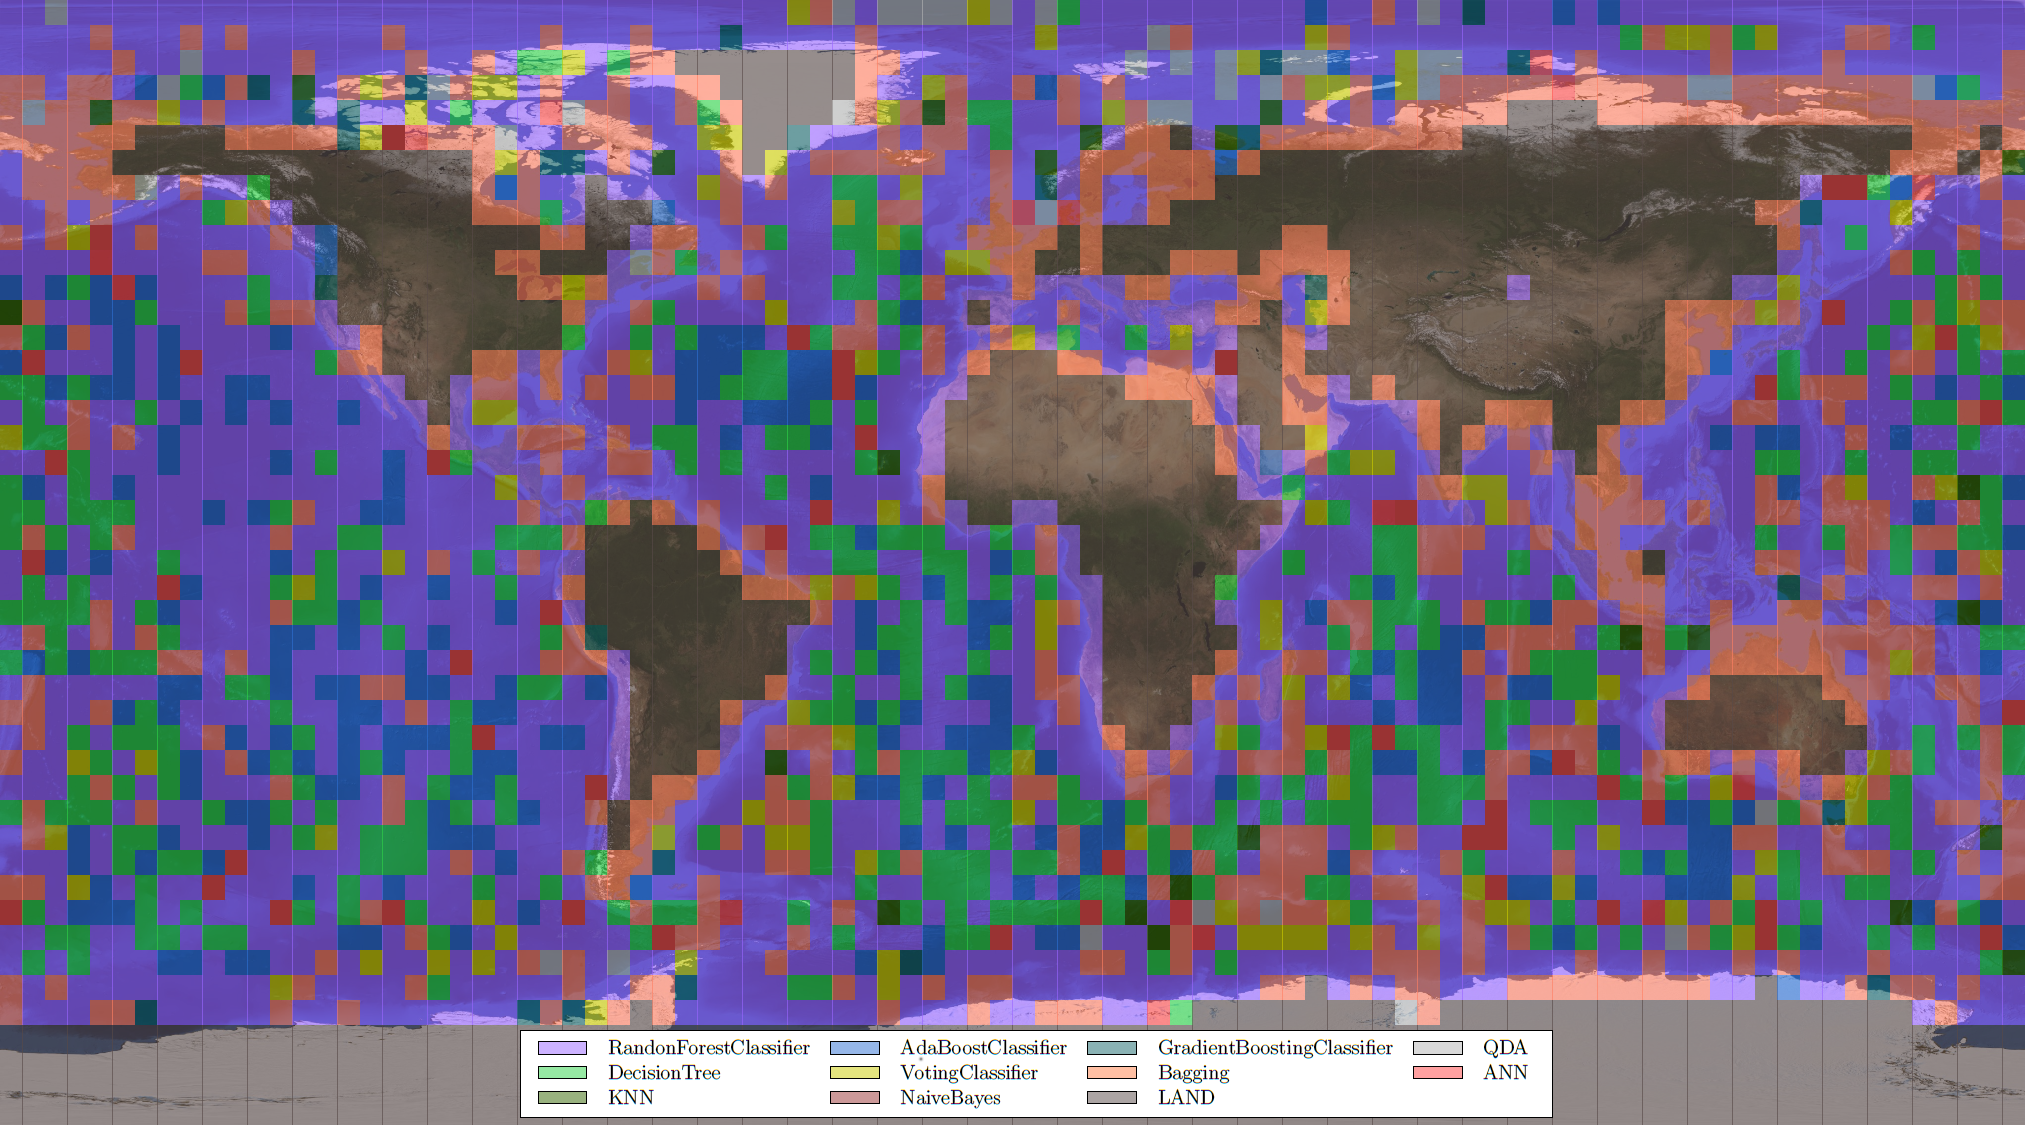
\includegraphics[width=\textwidth]{optgriddraft.png}
    \caption{Graphic Showing the World Coverages and Successful Models}
    \label{fig:coveragegrid}
\end{figure}

\par
This proof of concept was implemented and executed against the existing discrete classed bathymetry data used in the classification section.
A Python script iterated across a grid of the world and trained the set of models.
Then compared the trained models and selected the best performing model.
Figure \ref{fig:coveragegrid} shows the results of this script.
Clearly, there are consistencies in depth, fault lines, and coast lines for the best models.
This supports the idea that dynamically injecting models will locally boost accuracy.

%In this section I am defining what the Grid optimization is and why it matters.
%There may be a better name for this?? Who knows really...
\subsection{Grid Optimizing}
This concept was further implemented by partitioning the world into coverages.
These coverages mirror the partitioned areas used in figure \ref{fig:coveragegrid} for simplicity.
For this project, I trained a set of classification models on each coverage to predict bathymetry.
The model that most accurately predicted bathymetry was then recorded and stored into a data structure.
This structure is a simple map of a bounding boxes and models.

%This is where I define what happens after the appropriate coverages have been found.
\par
The map structure is then used to create an ensemble that selects the optimal model for predicting in a coverage.
I call this ensemble the \textit{Grid Optimized Model Injector Classifier}.
Each model is retrained and validated using a 10 fold cross validation on the worlds set of data.
This trained model is then persisted and stored for use in predictions.
The model injector then references the optimized grid map and injects the best model for that coverage.
This reference is a simple geospatial query for the latitude and longitude of the bathymetry point.

\par
In theory, this injection will allow each model to perform to its optimum.
Each coverage highlights distinct characteristics that perform better for a certain estimator.
There are several patterns that can be gleaned from figure \ref{fig:coveragegrid}. 
Such as: consistencies with depth, along fault lines, and potentially sediment composition. 
% Reconsider this sentence....


\subsection{Results and Metrics}
%The world wide ETOPO bathymetry dataset \cite{national1988etopo} at two minute resolution is used for valadation and metrics.
%This dataset is treated as the ground truth for all predictions.
%During the experiment, a one third holdout was used for validation in some cases.
%For finding the optimum model for a coverage a 10 fold cross validation was utilized.

%Include metrics information here.... possibly graphs and a list of scores? I dont really know.

%I dont like how I worded this whole section...
%The idea here is that I want to say "Hey, these people did this research and found the their regression model preforms poorly for predicting seamounts espicially after 500m.
%I clearly noticed a similar trend, but saw better preformance from some models than others. 
%This research is to identify those coverages and then use those results to build a super classifier.
%These metrics are important for identifying where the models preform well. 
The Grid Optimized Model Injector improved the accuracy of predictions by ~5\%.
These gains are made by leveraging the "strongest" classifier for a coverage.
The balanced accuracy was generated using 10 fold cross validation on the worlds set of data.
The average F1 score across classes was generated by training against the trainsets in figure \ref{fig:trainset} and validated against the rest of the world.
These results are displayed in table \ref{table:GRID_OPT_RESULTS}.

\begin{table}[htb]
    \begin{tabular}{|c c c|}
        \hline
        \textbf{Model} & \textbf{Average F1 Score} & \textbf{Mean Balanced Accuracy} \\
		\hline
		Grid Optimized Model Injector & 0.83 & 0.862 \\
		\hline
        \end{tabular}
        \label{table:GRID_OPT_RESULTS}
        \caption{Regression Results}
    \end{table}
\end{center}

%Extending off the research preformed in \cite{jena2012prediction} these metrics allow the selection of the best preforming model.

%Maybe here I can have a table show casing the preformance of models or possibly statistics about the coverages??
%It will be intersting to see what has preformed better across the globe
%Also is intersting to see which models have preformed best overall.
